% Why Machine Learning Strategy 
\chapter{机器学习策略}

\iffalse
Machine learning is the foundation of countless important applications, including web
search, email anti-spam, speech recognition, product recommendations, and more. I assume
that you or your team is working on a machine learning application, and that you want to
make rapid progress. This book will help you do so.
\fi

机器学习是很多重要应用的基础,
包括网页搜索,垃圾邮件识别,语音识别,推荐系统等等。
我假设,你和你的团队,正在做一个机器学习的应用,
并且你想快速进步,这本书会很好地帮助到你。

\iffalse
Example: Building a cat picture startup
Say you’re building a startup that will provide an endless stream of cat pictures to cat lovers.
You use a neural network to build a computer vision system for detecting cats in pictures
\fi

\textbf{以识别猫咪图片为例}

你想给广大铲屎官们提供可爱的猫咪图片,
你用神经网络搭建了一个计算机视觉系统来检测图片中的猫咪。
\begin{figure}[h]
	\centering
	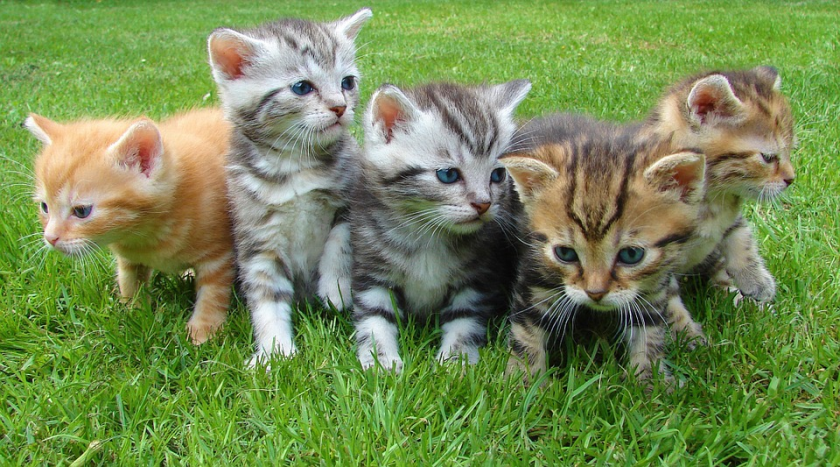
\includegraphics[width=0.7\linewidth]{TeX_files/pic/1.1}
	\caption{猫咪图片}
	\label{fig:1}
\end{figure}

\iffalse
But tragically, your learning algorithm’s accuracy is not yet good enough. You are under
tremendous pressure to improve your cat detector. What do you do?
Your team has a lot of ideas, such as:

• Get more data: Collect more pictures of cats.
• Collect a more diverse training set. For example, pictures of cats in unusual positions; cats
with unusual coloration; pictures shot with a variety of camera settings; ….
• Train the algorithm longer, by running more gradient descent iterations.
• Try a bigger neural network, with more layers/hidden units/parameters.
• Try a smaller neural network.
 Try adding regularization (such as L2 regularization).
• Change the neural network architecture (activation function, number of hidden units, etc.)
• …
\fi

但悲剧的是,你的算法准确率不够好,
你急切地想要改进你的猫咪检测器,
你打算怎么做?

你的团队可能会有如下的想法:
\begin{itemize}
	\item 获取更多的数据:收集更多的喵咪图片。
	\item 收集多样化的训练数据集。
	比如,图片中的猫咪处于特殊的位置;
	不同花色的猫咪;
	拍照时使用了不同设置的照片。
	\item 继续多训练一会,进行更多的梯度下降训练
	\item 采用更大的神经网络,增加隐藏层或节点数量或参数
	\item 尝试更小的神经网络
	\item 尝试增加正则项,如L2正则化
	\item 改变神经网络结构,如激励函数和隐藏节点数量等
	\item ...
	
\end{itemize}

\iffalse
If you choose well among these possible directions, you’ll build the leading cat picture
platform, and lead your company to success. If you choose poorly, you might waste months.
How do you proceed?
This book will tell you how. Most machine learning problems leave clues that tell you what’s
useful to try, and what’s not useful to try. Learning to read those clues will save you months
or years of development time.
\fi

如果你在这些可能的方向上作了较好得取舍,你会在识别猫咪上取得成功。
如果取舍得不好,你会白白浪费几个月。
那么你要如何进步呢?

这本书将会告诉你,大部分机器学习问题都会留下有用和没用的线索,
学会辨别这些线索,将会节省很多开发时间。


